%% LyX 1.6.5 created this file.  For more info, see http://www.lyx.org/.
%% Do not edit unless you really know what you are doing.
\documentclass[english]{article}
\usepackage[T1]{fontenc}
\usepackage[latin9]{inputenc}
\usepackage{graphicx}
\usepackage{babel}

\begin{document}

\title{Ping-Pong Design Documentation}


\author{Saurabh Kumar(2009cs10216)}

\maketitle
\newpage

\tableofcontents

\newpage


\section{What is being designed?}
\begin{itemize}
\item The design is basically an implementation of a networked multiplayered
game -Ping-Pong.
\item The game can be played by one player (against the computer), two players
(against each other with side walls bricked), three players (with
only one side of the screen bricked), and four players (the screen
is open on all four sides, and protected by the paddles of each player).
'bricked' means that the side is controlled by the computer. 
\item The game is played with a ball , paddles and a table like structure.The
ball moves on the table and the player's goal is to use the paddle
to prevent go past his/her side of the table and at the same time
making the ball run past his oppenents side.
\end{itemize}

\section{Game Flow:}
\begin{itemize}
\item When a player starts the game , game waits until other players ,if
any, also start the game and then the game begins with paddle of each
player in the middle of of their respective sides. 
\item On starting the game, the players can begin to navigate their paddles.
Meanwhile , the game records score of each player .When the time of
the game is over ,the game will end and the player with maximum score
will be the winner.
\item After that the game is finished the player can restart or quit the
game.During the game pressing Esc at any time will result in pausing
the game and returning to the main menu.
\item Pressing Esc button again will resume the game. Once a ball goes out
,the game will resume after some time delay. 
\end{itemize}

\section{Game Rules \& Player Controls:}
\begin{itemize}
\item Each match will be of prespecified game length in minutes .
\item Number of players :

\begin{itemize}
\item single player game \textendash{} against the computer 
\item two player game \textendash{} two players are on same or different
computers 
\item three player game \textendash{} one player is on server computer other
two on different computers (clients )
\item four player game \textendash{} one player is server and other three
on different computers (clients)
\end{itemize}
\item Scoreboard :

\begin{itemize}
\item Scoreboard shows number of miss by each player and time left.
\end{itemize}
\item Number of balls :

\begin{itemize}
\item Game can be played with one, two or three balls . 
\end{itemize}
\item Bricked walls :

\begin{itemize}
\item In case of multiplayer game, sides which are controlled by computer
with 100\% return probablity are bricked walls. Collision is elastic
with bricked walls. 
\end{itemize}
\item Ball reset : 

\begin{itemize}
\item Ball again comes in centre if ball goes out of outer field area. Initial
direction of ball is random. 
\end{itemize}
\item Controls 

\begin{enumerate}
\item move left : left arrow 
\item move right : right arrow 
\item hit : space bar 
\item pause : Esc
\end{enumerate}
If client and server play on same computer then client's controls
will be 
\begin{enumerate}
\item move left : a
\item move right:d
\item hit: s
\end{enumerate}

\paragraph*{\textmd{The player has to move the paddle along his/her side of the
table and occasionlly hit the ball. }}

\item Dimensions of table , paddles and ball are shown in the figure below.
\end{itemize}
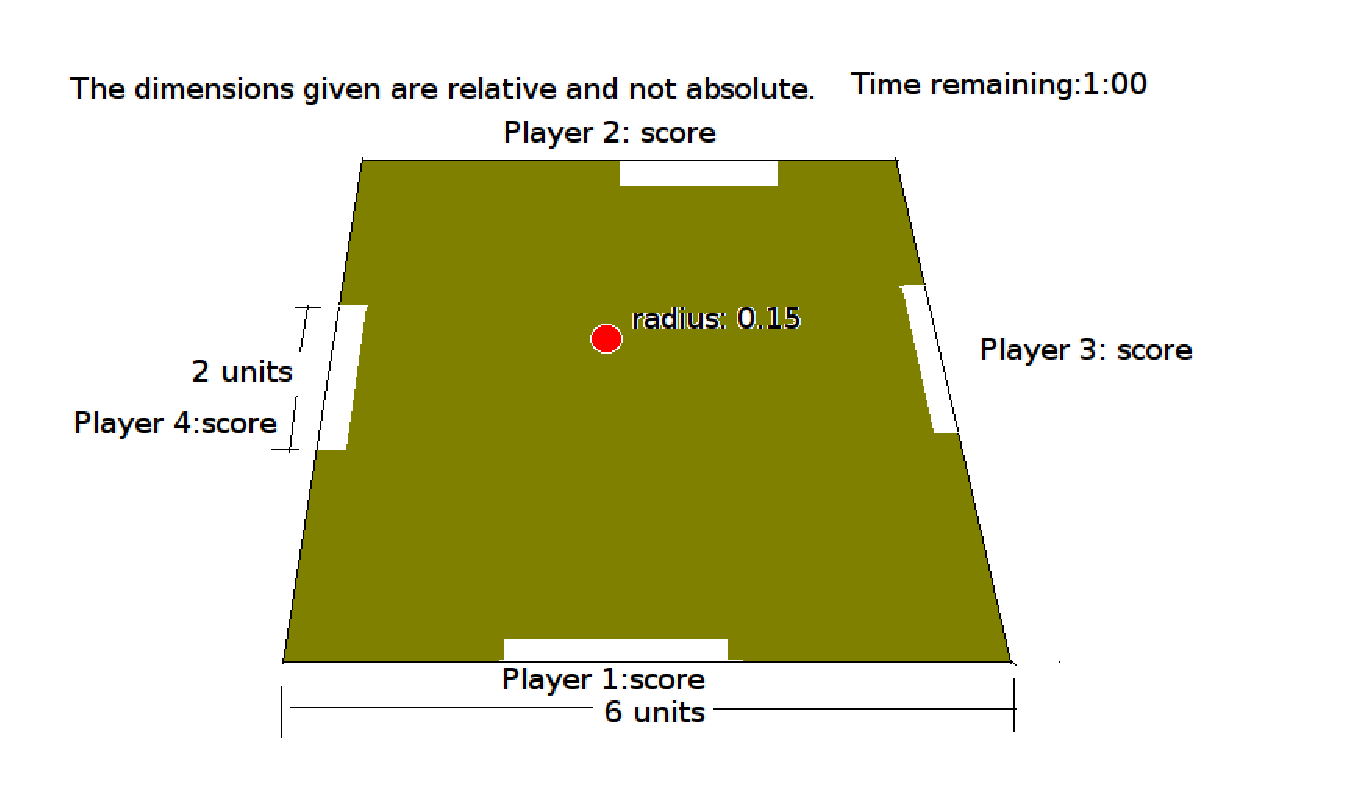
\includegraphics[bb=0bp 0bp 700bp 485bp,scale=0.5]{table}


\section{Technical features:}
\begin{itemize}
\item The coefficient of friction between the ball and the table can be
set to any value between 0 \& 0.1. 
\item The coefficient of restiution is different at different points on
paddle with maximum at the centre and minimum at the endpoint with
a linear variation. 
\item The ball will be given some velocity along the direction of motion
of the paddle. 
\item The power of shot will depend on the timing of the shot(i.e. Depends
on the time of pressing space bar).
\item Collision between the balls and the balls \& walls will be elastic. 
\end{itemize}

\section{Data \& State Abstractions}


\paragraph*{\textmd{We will use Object Oriented Programming to implement our
game.The important classes and structures include (with most likely
description)}}
\begin{itemize}
\item 'Game\_state' :
\end{itemize}

\subparagraph*{\textmd{struct Game\_state}}

\{

Player player1,player2,player3,player4;

Ball ball1,ball2,ball3;

....

\}
\begin{itemize}
\item 'Paddle' 
\end{itemize}

\subparagraph*{\textmd{class Paddle}}

\{

float coordinate;

float vel;

moveright()\{\}

move left()\{\}

..

\}
\begin{itemize}
\item 'Player' 
\end{itemize}

\subparagraph*{\textmd{class Player}}

\{

Paddle paddle;

int score;

increment\_score()\{\}

updatePaddle()\{\}

..

\}


\subparagraph*{\textmd{and }}
\begin{itemize}
\item 'Ball' 
\end{itemize}

\subparagraph*{\textmd{class Ball}}

\{

float x\_coord;

float y\_coord;

float x\_vel;

float y\_vel;

updateBall()

..

\}
\begin{itemize}
\item Client\_message etc.
\end{itemize}

\subparagraph{\textmd{struct Client\_message}}

\{

Paddle paddle;

int space\_pressed;

..

\}


\paragraph*{\textmd{The Game\_state struct is very important as this contains
the complete current state of the game that includes position and
velocity of all paddles and the balls and other game parameters. }}


\paragraph*{\textmd{If hosts stops sending messages ,it implies that the host
is inactive/down and we can display appropriate error messages.}}


\section{Client and Server :Parallel processing }
\begin{itemize}
\item To incorporate parallel processing that means that different players
can move their paddles parallely ,we use threads in server program
correspomding to different clients which handle different clients
in data transfer.So all the players will be able to move their paddles
parallely. 
\item The ball objects are updated by the server.
\item The server sends Game\_state structure to each of the client and the
clients send Client\_message structure to server after updating it.
\item Drawing graphics and listening to inputs for different players is
the responsibility of respective client programs.
\item The server and clients keep track of the scores , and stop the game
when either of the players win and display appropriate messages.
\item If server is temporarily away it may send some message and clients
will sleep until they receive some message from server.
\item In a one -player game ,server plays as the computer and a separate
client plays as the player.
\item In multiplayer games the server will play as one of the players.
\end{itemize}

\section{Network Protocol for network game}
\begin{itemize}
\item This game will use a TCP/IP network in order to create a multiplayer
match. When starting this game, one side is regarded as the server
(waiting for connections) and one is the client (connecting to the
server). The computer acting as the server will determine key game-parameters
such as friction coefficient,coefficient of restitution etc.
\item The communication of the client and server computers will be made
through messages. Each server-client message will be just the game
state structure while every client-server structure will be contain
state of paddle and whether 'space' button was pressed.
\item To connect client and server IP address of the server and the port
must be provided. (port number should genrally be greater than 1024).
\item For differnet clients ,server will have different threads listening
on different sockets to communicate parallely and at the same time
be able to distinguish among different clients' messages.
\item If hosts stops sending messages ,it implies that the host is inactive/down.
\item If a client does not responds , server will close the game.
\end{itemize}
The reasons we prefer TCP include that it is quite reliable and easy
to use.If we use UDP it might result in loss of packets which means
losing information.


\section{Graphics and Audio}

We will use OpenGL library to draw the graphical interface.
\begin{itemize}
\item Different clients will draw the tables, balls and all the paddles
with a suitable camera position using openGL for different players.
\item The glut window will show the game as well each player's score as
shown above in the figure.
\item For each player , his/her paddle will always be at the botttom most
edge of the table.
\item Double buffering will be used for smoother display and proper lighting
and texture will ensure a more natural look.
\item Messages appear on the screen to inform the player of the game's status. 
\item Suitable sounds will be played on important events like ball hitting
paddles,other collisions and other events like game over,victory etc.
\end{itemize}

\subsection{Graphical User Interface -GUI}
\begin{itemize}
\item Graphical User Interface include Static things like Ping Pong table
and Dynamic things like ball and paddles.
\item When a key is pressed, it calls a function in the application, called
a SpecialKeyFunction. When the application returns control to the
library, it calls the application's window redraw function. 
\item To ensure a smooth motion, key-press callbacks should not incrementally
update the orientation of the player's paddle. If this were the case,
the paddle would either move too slowly - as the user can only press
keys so fast -, or it would turn in large, visibly discrete, steps.
Instead, key-press callbacks will set global variables, indicating
a request such as \textquotedbl{}the user wishes to move right\textquotedbl{}.
These variables remain set until the user releases the key. While
the key is held down, and the corresponding global variables are set,
the player's paddle moves slightly every time the game board is updated.
\end{itemize}

\section{Executing the game program}
\begin{itemize}
\item System requirements: openGL library,g++ compiler and runtime environment.
\item game help


\$ make help will show a short help screen .

\item Create a parameter file. This is a text file containing the desired
setup of PingPong. The parameters include :

\begin{enumerate}
\item Server IP
\item Port Number
\item Number of players
\item Number of balls
\item Duration of the game
\item Hardness level........
\end{enumerate}
\end{itemize}
\begin{enumerate}
\item Execute game as : 

\begin{enumerate}
\item \$make all (Compile your project)
\item \$ make server ( if you are a server )
\item \$ make client ( if you are a client )
\item \$ make game ( if two player play on same computer )
\item \$ make server ( to play a single player game and specify no. of players
=1 in parameter file)
\item \$ make computer ( to see match between both computer players)
\item \$ make test1, make test2, make test3, ... will run the respective
tests
\end{enumerate}
\end{enumerate}

\section{Tests}
\begin{itemize}
\item Test by playing a computer against another computer. Test in the following
scenarios: 

\begin{itemize}
\item Both players are on the same computer and use your implementation 
\item Both players are on different computers and use your implementation 
\item Both players are on the same computer and one player uses your implementation
and the other player uses your partner's implementation 
\item Both players are on different computers and one player uses your implementation
and the other player uses your partner's implementation 
\end{itemize}
\item Play with one ball, two balls, and three balls. 
\end{itemize}

\section{Interesting features that may be imparted to the game}
\begin{itemize}
\item The pre-game gui, the in-game-help gui and the end-game gui.

\begin{enumerate}
\item The pre-game GUI is a simple menu system which is controlled by mouse
input, and gives access to starting a new game, the single and multiplayer
game gui, an about gui embedded in it that gives information about
the game and information about the controls, and a quit button. 
\item The in-game-help gui will provide the user a chance to access controls
information about the game. This will be implemented as a game pausing
feature with a menu that pops up in the middle of the screen for easy
reading.
\item The end-game gui will give users choice to restart game or simply
quit the game.
\end{enumerate}
\item Freedom to change view: The user can view the table at different angles
customised to his likes.
\end{itemize}

\end{document}
